%%%%%%%%%%%%%%%%%%%%%%%%%%%%%%%%%%%%%%%%%
% The Legrand Orange Book
% LaTeX Template
% Version 2.4 (26/09/2018)
%
% This template was downloaded from:
% http://www.LaTeXTemplates.com
%
% Original author:
% Mathias Legrand (legrand.mathias@gmail.com) with modifications by:
% Vel (vel@latextemplates.com)
%
% License:
% CC BY-NC-SA 3.0 (http://creativecommons.org/licenses/by-nc-sa/3.0/)
%
% Compiling this template:
% This template uses biber for its bibliography and makeindex for its index.
% When you first open the template, compile it from the command line with the 
% commands below to make sure your LaTeX distribution is configured correctly:
%
% 1) pdflatex main
% 2) makeindex main.idx -s StyleInd.ist
% 3) biber main
% 4) pdflatex main x 2
%
% After this, when you wish to update the bibliography/index use the appropriate
% command above and make sure to compile with pdflatex several times 
% afterwards to propagate your changes to the document.
%
% This template also uses a number of packages which may need to be
% updated to the newest versions for the template to compile. It is strongly
% recommended you update your LaTeX distribution if you have any
% compilation errors.
%
% Important note:
% Chapter heading images should have a 2:1 width:height ratio,
% e.g. 920px width and 460px height.
%
%%%%%%%%%%%%%%%%%%%%%%%%%%%%%%%%%%%%%%%%%

%----------------------------------------------------------------------------------------
%	PACKAGES AND OTHER DOCUMENT CONFIGURATIONS
%----------------------------------------------------------------------------------------

\documentclass[11pt,fleqn]{book} % Default font size and left-justified equations

%%%%%%%%%%%%%%%%%%%%%%%%%%%%%%%%%%%%%%%%%
% The Legrand Orange Book
% Structural Definitions File
% Version 2.1 (26/09/2018)
%
% Original author:
% Mathias Legrand (legrand.mathias@gmail.com) with modifications by:
% Vel (vel@latextemplates.com)
% 
% This file was downloaded from:
% http://www.LaTeXTemplates.com
%
% License:
% CC BY-NC-SA 3.0 (http://creativecommons.org/licenses/by-nc-sa/3.0/)
%
%%%%%%%%%%%%%%%%%%%%%%%%%%%%%%%%%%%%%%%%%

%----------------------------------------------------------------------------------------
%	VARIOUS REQUIRED PACKAGES AND CONFIGURATIONS
%----------------------------------------------------------------------------------------

\usepackage{graphicx} % Required for including pictures
\graphicspath{{Pictures/}} % Specifies the directory where pictures are stored

\usepackage{lipsum} % Inserts dummy text

\usepackage{tikz} % Required for drawing custom shapes

\usepackage[english]{babel} % English language/hyphenation

\usepackage{enumitem} % Customize lists
\setlist{nolistsep} % Reduce spacing between bullet points and numbered lists

\usepackage{booktabs} % Required for nicer horizontal rules in tables

\usepackage{xcolor} % Required for specifying colors by name
\definecolor{ocre}{RGB}{243,102,25} % Define the orange color used for highlighting throughout the book

%----------------------------------------------------------------------------------------
%	MARGINS
%----------------------------------------------------------------------------------------

\usepackage{geometry} % Required for adjusting page dimensions and margins

\geometry{
	paper=a4paper, % Paper size, change to letterpaper for US letter size
	top=3cm, % Top margin
	bottom=3cm, % Bottom margin
	left=3cm, % Left margin
	right=3cm, % Right margin
	headheight=14pt, % Header height
	footskip=1.4cm, % Space from the bottom margin to the baseline of the footer
	headsep=10pt, % Space from the top margin to the baseline of the header
	%showframe, % Uncomment to show how the type block is set on the page
}

%----------------------------------------------------------------------------------------
%	FONTS
%----------------------------------------------------------------------------------------

\usepackage{avant} % Use the Avantgarde font for headings
%\usepackage{times} % Use the Times font for headings
\usepackage{mathptmx} % Use the Adobe Times Roman as the default text font together with math symbols from the Sym­bol, Chancery and Com­puter Modern fonts

\usepackage{microtype} % Slightly tweak font spacing for aesthetics
\usepackage[utf8]{inputenc} % Required for including letters with accents
\usepackage[T1]{fontenc} % Use 8-bit encoding that has 256 glyphs

%----------------------------------------------------------------------------------------
%	BIBLIOGRAPHY AND INDEX
%----------------------------------------------------------------------------------------

\usepackage[style=numeric,citestyle=numeric,sorting=nyt,sortcites=true,autopunct=true,babel=hyphen,hyperref=true,abbreviate=false,backref=true,backend=biber]{biblatex}
\addbibresource{bibliography.bib} % BibTeX bibliography file
\defbibheading{bibempty}{}

\usepackage{calc} % For simpler calculation - used for spacing the index letter headings correctly
\usepackage{makeidx} % Required to make an index
\makeindex % Tells LaTeX to create the files required for indexing

%----------------------------------------------------------------------------------------
%	MAIN TABLE OF CONTENTS
%----------------------------------------------------------------------------------------

\usepackage{titletoc} % Required for manipulating the table of contents

\contentsmargin{0cm} % Removes the default margin

% Part text styling (this is mostly taken care of in the PART HEADINGS section of this file)
\titlecontents{part}
	[0cm] % Left indentation
	{\addvspace{20pt}\bfseries} % Spacing and font options for parts
	{}
	{}
	{}

% Chapter text styling
\titlecontents{chapter}
	[1.25cm] % Left indentation
	{\addvspace{12pt}\large\sffamily\bfseries} % Spacing and font options for chapters
	{\color{ocre!60}\contentslabel[\Large\thecontentslabel]{1.25cm}\color{ocre}} % Formatting of numbered sections of this type
	{\color{ocre}} % Formatting of numberless sections of this type
	{\color{ocre!60}\normalsize\;\titlerule*[.5pc]{.}\;\thecontentspage} % Formatting of the filler to the right of the heading and the page number

% Section text styling
\titlecontents{section}
	[1.25cm] % Left indentation
	{\addvspace{3pt}\sffamily\bfseries} % Spacing and font options for sections
	{\contentslabel[\thecontentslabel]{1.25cm}} % Formatting of numbered sections of this type
	{} % Formatting of numberless sections of this type
	{\hfill\color{black}\thecontentspage} % Formatting of the filler to the right of the heading and the page number

% Subsection text styling
\titlecontents{subsection}
	[1.25cm] % Left indentation
	{\addvspace{1pt}\sffamily\small} % Spacing and font options for subsections
	{\contentslabel[\thecontentslabel]{1.25cm}} % Formatting of numbered sections of this type
	{} % Formatting of numberless sections of this type
	{\ \titlerule*[.5pc]{.}\;\thecontentspage} % Formatting of the filler to the right of the heading and the page number

% Figure text styling
\titlecontents{figure}
	[1.25cm] % Left indentation
	{\addvspace{1pt}\sffamily\small} % Spacing and font options for figures
	{\thecontentslabel\hspace*{1em}} % Formatting of numbered sections of this type
	{} % Formatting of numberless sections of this type
	{\ \titlerule*[.5pc]{.}\;\thecontentspage} % Formatting of the filler to the right of the heading and the page number

% Table text styling
\titlecontents{table}
	[1.25cm] % Left indentation
	{\addvspace{1pt}\sffamily\small} % Spacing and font options for tables
	{\thecontentslabel\hspace*{1em}} % Formatting of numbered sections of this type
	{} % Formatting of numberless sections of this type
	{\ \titlerule*[.5pc]{.}\;\thecontentspage} % Formatting of the filler to the right of the heading and the page number

%----------------------------------------------------------------------------------------
%	MINI TABLE OF CONTENTS IN PART HEADS
%----------------------------------------------------------------------------------------

% Chapter text styling
\titlecontents{lchapter}
	[0em] % Left indentation
	{\addvspace{15pt}\large\sffamily\bfseries} % Spacing and font options for chapters
	{\color{ocre}\contentslabel[\Large\thecontentslabel]{1.25cm}\color{ocre}} % Chapter number
	{}  
	{\color{ocre}\normalsize\sffamily\bfseries\;\titlerule*[.5pc]{.}\;\thecontentspage} % Page number

% Section text styling
\titlecontents{lsection}
	[0em] % Left indentation
	{\sffamily\small} % Spacing and font options for sections
	{\contentslabel[\thecontentslabel]{1.25cm}} % Section number
	{}
	{}

% Subsection text styling (note these aren't shown by default, display them by searchings this file for tocdepth and reading the commented text)
\titlecontents{lsubsection}
	[.5em] % Left indentation
	{\sffamily\footnotesize} % Spacing and font options for subsections
	{\contentslabel[\thecontentslabel]{1.25cm}}
	{}
	{}

%----------------------------------------------------------------------------------------
%	HEADERS AND FOOTERS
%----------------------------------------------------------------------------------------

\usepackage{fancyhdr} % Required for header and footer configuration

\pagestyle{fancy} % Enable the custom headers and footers

\renewcommand{\chaptermark}[1]{\markboth{\sffamily\normalsize\bfseries\chaptername\ \thechapter.\ #1}{}} % Styling for the current chapter in the header
\renewcommand{\sectionmark}[1]{\markright{\sffamily\normalsize\thesection\hspace{5pt}#1}{}} % Styling for the current section in the header

\fancyhf{} % Clear default headers and footers
\fancyhead[LE,RO]{\sffamily\normalsize\thepage} % Styling for the page number in the header
\fancyhead[LO]{\rightmark} % Print the nearest section name on the left side of odd pages
\fancyhead[RE]{\leftmark} % Print the current chapter name on the right side of even pages
%\fancyfoot[C]{\thepage} % Uncomment to include a footer

\renewcommand{\headrulewidth}{0.5pt} % Thickness of the rule under the header

\fancypagestyle{plain}{% Style for when a plain pagestyle is specified
	\fancyhead{}\renewcommand{\headrulewidth}{0pt}%
}

% Removes the header from odd empty pages at the end of chapters
\makeatletter
\renewcommand{\cleardoublepage}{
\clearpage\ifodd\c@page\else
\hbox{}
\vspace*{\fill}
\thispagestyle{empty}
\newpage
\fi}

%----------------------------------------------------------------------------------------
%	THEOREM STYLES
%----------------------------------------------------------------------------------------

\usepackage{amsmath,amsfonts,amssymb,amsthm} % For math equations, theorems, symbols, etc

\newcommand{\intoo}[2]{\mathopen{]}#1\,;#2\mathclose{[}}
\newcommand{\ud}{\mathop{\mathrm{{}d}}\mathopen{}}
\newcommand{\intff}[2]{\mathopen{[}#1\,;#2\mathclose{]}}
\renewcommand{\qedsymbol}{$\blacksquare$}
\newtheorem{notation}{Notation}[chapter]

% Boxed/framed environments
\newtheoremstyle{ocrenumbox}% Theorem style name
{0pt}% Space above
{0pt}% Space below
{\normalfont}% Body font
{}% Indent amount
{\small\bf\sffamily\color{ocre}}% Theorem head font
{\;}% Punctuation after theorem head
{0.25em}% Space after theorem head
{\small\sffamily\color{ocre}\thmname{#1}\nobreakspace\thmnumber{\@ifnotempty{#1}{}\@upn{#2}}% Theorem text (e.g. Theorem 2.1)
\thmnote{\nobreakspace\the\thm@notefont\sffamily\bfseries\color{black}---\nobreakspace#3.}} % Optional theorem note

\newtheoremstyle{blacknumex}% Theorem style name
{5pt}% Space above
{5pt}% Space below
{\normalfont}% Body font
{} % Indent amount
{\small\bf\sffamily}% Theorem head font
{\;}% Punctuation after theorem head
{0.25em}% Space after theorem head
{\small\sffamily{\tiny\ensuremath{\blacksquare}}\nobreakspace\thmname{#1}\nobreakspace\thmnumber{\@ifnotempty{#1}{}\@upn{#2}}% Theorem text (e.g. Theorem 2.1)
\thmnote{\nobreakspace\the\thm@notefont\sffamily\bfseries---\nobreakspace#3.}}% Optional theorem note

\newtheoremstyle{blacknumbox} % Theorem style name
{0pt}% Space above
{0pt}% Space below
{\normalfont}% Body font
{}% Indent amount
{\small\bf\sffamily}% Theorem head font
{\;}% Punctuation after theorem head
{0.25em}% Space after theorem head
{\small\sffamily\thmname{#1}\nobreakspace\thmnumber{\@ifnotempty{#1}{}\@upn{#2}}% Theorem text (e.g. Theorem 2.1)
\thmnote{\nobreakspace\the\thm@notefont\sffamily\bfseries---\nobreakspace#3.}}% Optional theorem note

% Non-boxed/non-framed environments
\newtheoremstyle{ocrenum}% Theorem style name
{5pt}% Space above
{5pt}% Space below
{\normalfont}% Body font
{}% Indent amount
{\small\bf\sffamily\color{ocre}}% Theorem head font
{\;}% Punctuation after theorem head
{0.25em}% Space after theorem head
{\small\sffamily\color{ocre}\thmname{#1}\nobreakspace\thmnumber{\@ifnotempty{#1}{}\@upn{#2}}% Theorem text (e.g. Theorem 2.1)
\thmnote{\nobreakspace\the\thm@notefont\sffamily\bfseries\color{black}---\nobreakspace#3.}} % Optional theorem note
\makeatother

% Defines the theorem text style for each type of theorem to one of the three styles above
\newcounter{dummy} 
\numberwithin{dummy}{section}
\theoremstyle{ocrenumbox}
\newtheorem{theoremeT}[dummy]{Theorem}
\newtheorem{problem}{Problem}[chapter]
\newtheorem{exerciseT}{Exercise}[chapter]
\theoremstyle{blacknumex}
\newtheorem{exampleT}{Example}[chapter]
\theoremstyle{blacknumbox}
\newtheorem{vocabulary}{Vocabulary}[chapter]
\newtheorem{definitionT}{Definition}[section]
\newtheorem{corollaryT}[dummy]{Corollary}
\theoremstyle{ocrenum}
\newtheorem{proposition}[dummy]{Proposition}

%----------------------------------------------------------------------------------------
%	DEFINITION OF COLORED BOXES
%----------------------------------------------------------------------------------------

\RequirePackage[framemethod=default]{mdframed} % Required for creating the theorem, definition, exercise and corollary boxes

% Theorem box
\newmdenv[skipabove=7pt,
skipbelow=7pt,
backgroundcolor=black!5,
linecolor=ocre,
innerleftmargin=5pt,
innerrightmargin=5pt,
innertopmargin=5pt,
leftmargin=0cm,
rightmargin=0cm,
innerbottommargin=5pt]{tBox}

% Exercise box	  
\newmdenv[skipabove=7pt,
skipbelow=7pt,
rightline=false,
leftline=true,
topline=false,
bottomline=false,
backgroundcolor=ocre!10,
linecolor=ocre,
innerleftmargin=5pt,
innerrightmargin=5pt,
innertopmargin=5pt,
innerbottommargin=5pt,
leftmargin=0cm,
rightmargin=0cm,
linewidth=4pt]{eBox}	

% Definition box
\newmdenv[skipabove=7pt,
skipbelow=7pt,
rightline=false,
leftline=true,
topline=false,
bottomline=false,
linecolor=ocre,
innerleftmargin=5pt,
innerrightmargin=5pt,
innertopmargin=0pt,
leftmargin=0cm,
rightmargin=0cm,
linewidth=4pt,
innerbottommargin=0pt]{dBox}	

% Corollary box
\newmdenv[skipabove=7pt,
skipbelow=7pt,
rightline=false,
leftline=true,
topline=false,
bottomline=false,
linecolor=gray,
backgroundcolor=black!5,
innerleftmargin=5pt,
innerrightmargin=5pt,
innertopmargin=5pt,
leftmargin=0cm,
rightmargin=0cm,
linewidth=4pt,
innerbottommargin=5pt]{cBox}

% Creates an environment for each type of theorem and assigns it a theorem text style from the "Theorem Styles" section above and a colored box from above
\newenvironment{theorem}{\begin{tBox}\begin{theoremeT}}{\end{theoremeT}\end{tBox}}
\newenvironment{exercise}{\begin{eBox}\begin{exerciseT}}{\hfill{\color{ocre}\tiny\ensuremath{\blacksquare}}\end{exerciseT}\end{eBox}}				  
\newenvironment{definition}{\begin{dBox}\begin{definitionT}}{\end{definitionT}\end{dBox}}	
\newenvironment{example}{\begin{exampleT}}{\hfill{\tiny\ensuremath{\blacksquare}}\end{exampleT}}		
\newenvironment{corollary}{\begin{cBox}\begin{corollaryT}}{\end{corollaryT}\end{cBox}}	

%----------------------------------------------------------------------------------------
%	REMARK ENVIRONMENT
%----------------------------------------------------------------------------------------

\newenvironment{remark}{\par\vspace{10pt}\small % Vertical white space above the remark and smaller font size
\begin{list}{}{
\leftmargin=35pt % Indentation on the left
\rightmargin=25pt}\item\ignorespaces % Indentation on the right
\makebox[-2.5pt]{\begin{tikzpicture}[overlay]
\node[draw=ocre!60,line width=1pt,circle,fill=ocre!25,font=\sffamily\bfseries,inner sep=2pt,outer sep=0pt] at (-15pt,0pt){\textcolor{ocre}{R}};\end{tikzpicture}} % Orange R in a circle
\advance\baselineskip -1pt}{\end{list}\vskip5pt} % Tighter line spacing and white space after remark

%----------------------------------------------------------------------------------------
%	SECTION NUMBERING IN THE MARGIN
%----------------------------------------------------------------------------------------

\makeatletter
\renewcommand{\@seccntformat}[1]{\llap{\textcolor{ocre}{\csname the#1\endcsname}\hspace{1em}}}                    
\renewcommand{\section}{\@startsection{section}{1}{\z@}
{-4ex \@plus -1ex \@minus -.4ex}
{1ex \@plus.2ex }
{\normalfont\large\sffamily\bfseries}}
\renewcommand{\subsection}{\@startsection {subsection}{2}{\z@}
{-3ex \@plus -0.1ex \@minus -.4ex}
{0.5ex \@plus.2ex }
{\normalfont\sffamily\bfseries}}
\renewcommand{\subsubsection}{\@startsection {subsubsection}{3}{\z@}
{-2ex \@plus -0.1ex \@minus -.2ex}
{.2ex \@plus.2ex }
{\normalfont\small\sffamily\bfseries}}                        
\renewcommand\paragraph{\@startsection{paragraph}{4}{\z@}
{-2ex \@plus-.2ex \@minus .2ex}
{.1ex}
{\normalfont\small\sffamily\bfseries}}

%----------------------------------------------------------------------------------------
%	PART HEADINGS
%----------------------------------------------------------------------------------------

% Numbered part in the table of contents
\newcommand{\@mypartnumtocformat}[2]{%
	\setlength\fboxsep{0pt}%
	\noindent\colorbox{ocre!20}{\strut\parbox[c][.7cm]{\ecart}{\color{ocre!70}\Large\sffamily\bfseries\centering#1}}\hskip\esp\colorbox{ocre!40}{\strut\parbox[c][.7cm]{\linewidth-\ecart-\esp}{\Large\sffamily\centering#2}}%
}

% Unnumbered part in the table of contents
\newcommand{\@myparttocformat}[1]{%
	\setlength\fboxsep{0pt}%
	\noindent\colorbox{ocre!40}{\strut\parbox[c][.7cm]{\linewidth}{\Large\sffamily\centering#1}}%
}

\newlength\esp
\setlength\esp{4pt}
\newlength\ecart
\setlength\ecart{1.2cm-\esp}
\newcommand{\thepartimage}{}%
\newcommand{\partimage}[1]{\renewcommand{\thepartimage}{#1}}%
\def\@part[#1]#2{%
\ifnum \c@secnumdepth >-2\relax%
\refstepcounter{part}%
\addcontentsline{toc}{part}{\texorpdfstring{\protect\@mypartnumtocformat{\thepart}{#1}}{\partname~\thepart\ ---\ #1}}
\else%
\addcontentsline{toc}{part}{\texorpdfstring{\protect\@myparttocformat{#1}}{#1}}%
\fi%
\startcontents%
\markboth{}{}%
{\thispagestyle{empty}%
\begin{tikzpicture}[remember picture,overlay]%
\node at (current page.north west){\begin{tikzpicture}[remember picture,overlay]%	
\fill[ocre!20](0cm,0cm) rectangle (\paperwidth,-\paperheight);
\node[anchor=north] at (4cm,-3.25cm){\color{ocre!40}\fontsize{220}{100}\sffamily\bfseries\thepart}; 
\node[anchor=south east] at (\paperwidth-1cm,-\paperheight+1cm){\parbox[t][][t]{8.5cm}{
\printcontents{l}{0}{\setcounter{tocdepth}{1}}% The depth to which the Part mini table of contents displays headings; 0 for chapters only, 1 for chapters and sections and 2 for chapters, sections and subsections
}};
\node[anchor=north east] at (\paperwidth-1.5cm,-3.25cm){\parbox[t][][t]{15cm}{\strut\raggedleft\color{white}\fontsize{30}{30}\sffamily\bfseries#2}};
\end{tikzpicture}};
\end{tikzpicture}}%
\@endpart}
\def\@spart#1{%
\startcontents%
\phantomsection
{\thispagestyle{empty}%
\begin{tikzpicture}[remember picture,overlay]%
\node at (current page.north west){\begin{tikzpicture}[remember picture,overlay]%	
\fill[ocre!20](0cm,0cm) rectangle (\paperwidth,-\paperheight);
\node[anchor=north east] at (\paperwidth-1.5cm,-3.25cm){\parbox[t][][t]{15cm}{\strut\raggedleft\color{white}\fontsize{30}{30}\sffamily\bfseries#1}};
\end{tikzpicture}};
\end{tikzpicture}}
\addcontentsline{toc}{part}{\texorpdfstring{%
\setlength\fboxsep{0pt}%
\noindent\protect\colorbox{ocre!40}{\strut\protect\parbox[c][.7cm]{\linewidth}{\Large\sffamily\protect\centering #1\quad\mbox{}}}}{#1}}%
\@endpart}
\def\@endpart{\vfil\newpage
\if@twoside
\if@openright
\null
\thispagestyle{empty}%
\newpage
\fi
\fi
\if@tempswa
\twocolumn
\fi}

%----------------------------------------------------------------------------------------
%	CHAPTER HEADINGS
%----------------------------------------------------------------------------------------

% A switch to conditionally include a picture, implemented by Christian Hupfer
\newif\ifusechapterimage
\usechapterimagetrue
\newcommand{\thechapterimage}{}%
\newcommand{\chapterimage}[1]{\ifusechapterimage\renewcommand{\thechapterimage}{#1}\fi}%
\newcommand{\autodot}{.}
\def\@makechapterhead#1{%
{\parindent \z@ \raggedright \normalfont
\ifnum \c@secnumdepth >\m@ne
\if@mainmatter
\begin{tikzpicture}[remember picture,overlay]
\node at (current page.north west)
{\begin{tikzpicture}[remember picture,overlay]
\node[anchor=north west,inner sep=0pt] at (0,0) {\ifusechapterimage\includegraphics[width=\paperwidth]{\thechapterimage}\fi};
\draw[anchor=west] (\Gm@lmargin,-9cm) node [line width=2pt,rounded corners=15pt,draw=ocre,fill=white,fill opacity=0.5,inner sep=15pt]{\strut\makebox[22cm]{}};
\draw[anchor=west] (\Gm@lmargin+.3cm,-9cm) node {\huge\sffamily\bfseries\color{black}\thechapter\autodot~#1\strut};
\end{tikzpicture}};
\end{tikzpicture}
\else
\begin{tikzpicture}[remember picture,overlay]
\node at (current page.north west)
{\begin{tikzpicture}[remember picture,overlay]
\node[anchor=north west,inner sep=0pt] at (0,0) {\ifusechapterimage\includegraphics[width=\paperwidth]{\thechapterimage}\fi};
\draw[anchor=west] (\Gm@lmargin,-9cm) node [line width=2pt,rounded corners=15pt,draw=ocre,fill=white,fill opacity=0.5,inner sep=15pt]{\strut\makebox[22cm]{}};
\draw[anchor=west] (\Gm@lmargin+.3cm,-9cm) node {\huge\sffamily\bfseries\color{black}#1\strut};
\end{tikzpicture}};
\end{tikzpicture}
\fi\fi\par\vspace*{270\p@}}}

%-------------------------------------------

\def\@makeschapterhead#1{%
\begin{tikzpicture}[remember picture,overlay]
\node at (current page.north west)
{\begin{tikzpicture}[remember picture,overlay]
\node[anchor=north west,inner sep=0pt] at (0,0) {\ifusechapterimage\includegraphics[width=\paperwidth]{\thechapterimage}\fi};
\draw[anchor=west] (\Gm@lmargin,-9cm) node [line width=2pt,rounded corners=15pt,draw=ocre,fill=white,fill opacity=0.5,inner sep=15pt]{\strut\makebox[22cm]{}};
\draw[anchor=west] (\Gm@lmargin+.3cm,-9cm) node {\huge\sffamily\bfseries\color{black}#1\strut};
\end{tikzpicture}};
\end{tikzpicture}
\par\vspace*{270\p@}}
\makeatother

%----------------------------------------------------------------------------------------
%	LINKS
%----------------------------------------------------------------------------------------

\usepackage{hyperref}
\hypersetup{hidelinks,backref=true,pagebackref=true,hyperindex=true,colorlinks=false,breaklinks=true,urlcolor=ocre,bookmarks=true,bookmarksopen=false}

\usepackage{bookmark}
\bookmarksetup{
open,
numbered,
addtohook={%
\ifnum\bookmarkget{level}=0 % chapter
\bookmarksetup{bold}%
\fi
\ifnum\bookmarkget{level}=-1 % part
\bookmarksetup{color=ocre,bold}%
\fi
}
}
 % Insert the commands.tex file which contains the majority of the structure behind the template

%\hypersetup{pdftitle={Title},pdfauthor={Author}} % Uncomment and fill out to include PDF metadata for the author and title of the book

%----------------------------------------------------------------------------------------

\begin{document}

%----------------------------------------------------------------------------------------
%	TITLE PAGE
%----------------------------------------------------------------------------------------

\begingroup
\thispagestyle{empty} % Suppress headers and footers on the title page
\begin{tikzpicture}[remember picture,overlay]
\node[inner sep=0pt] (background) at (current page.center) {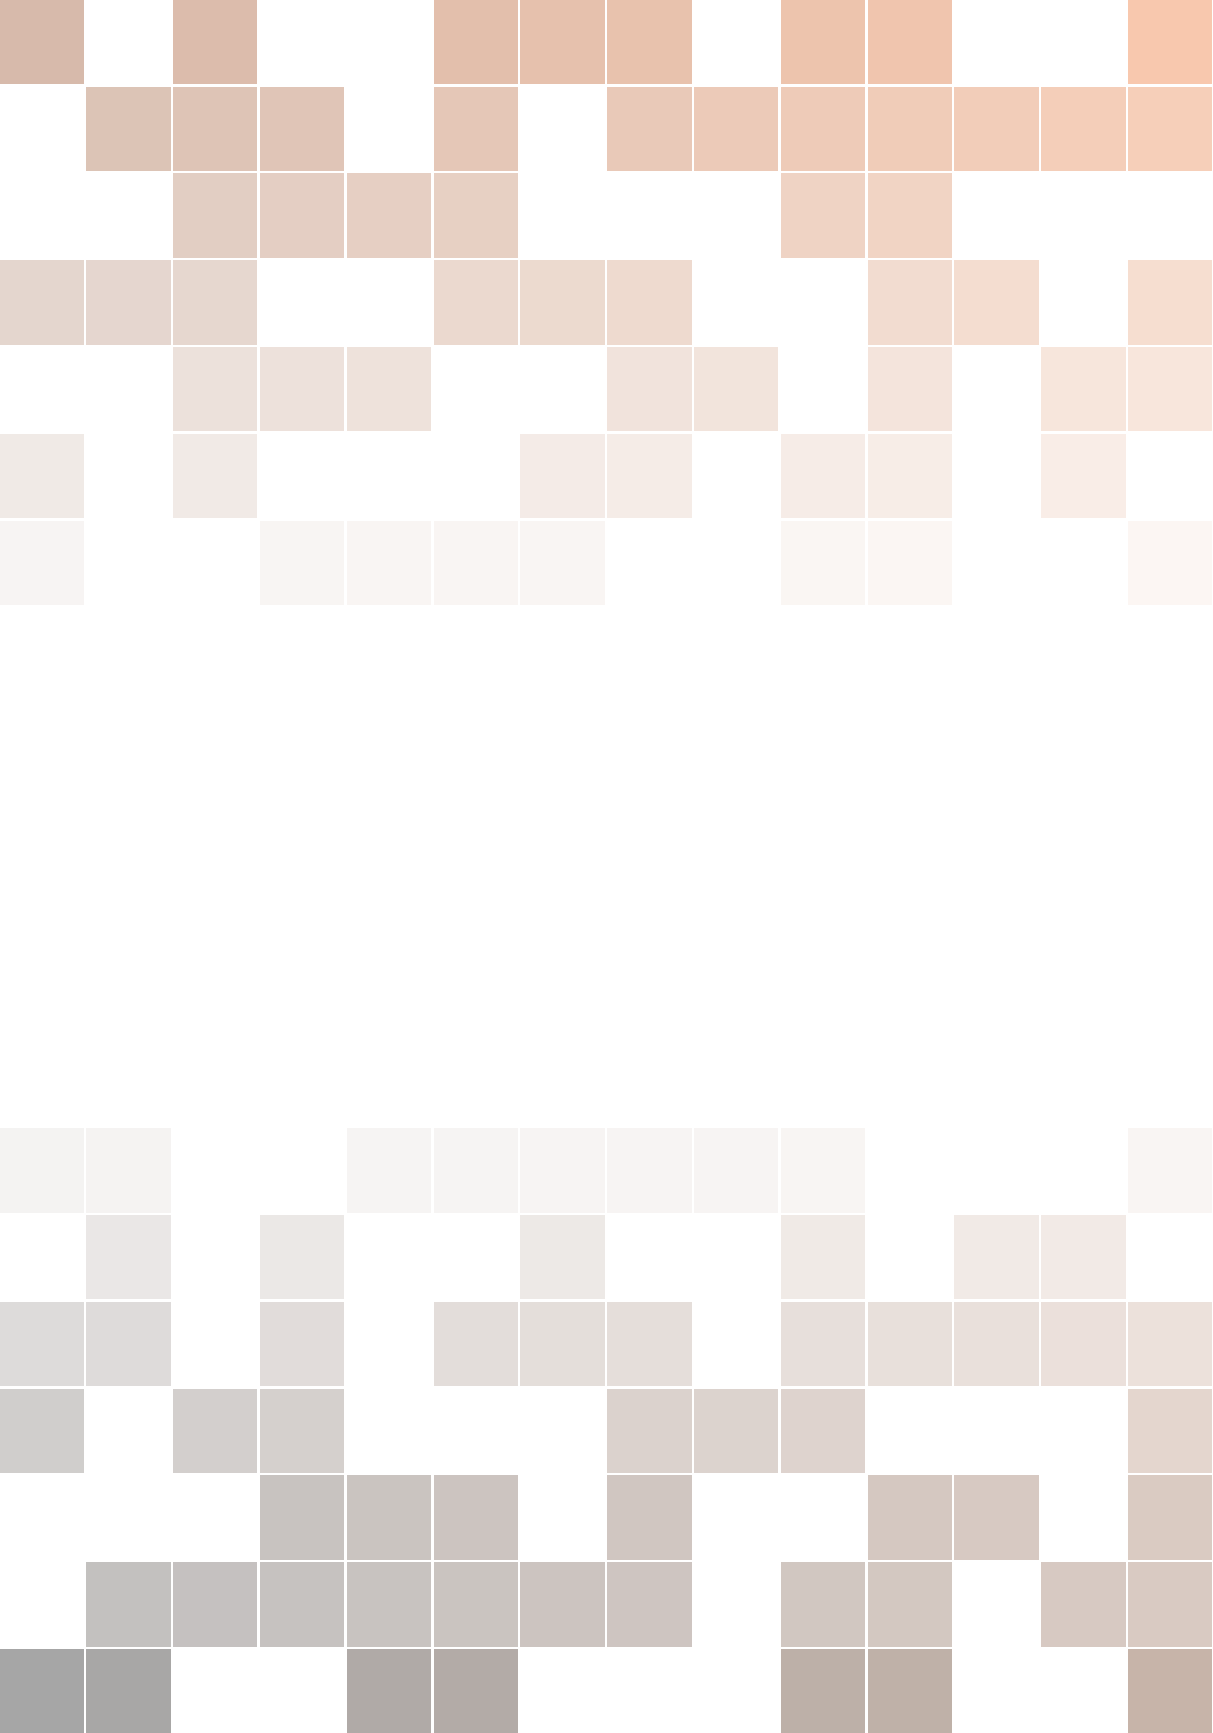
\includegraphics[width=\paperwidth]{background.pdf}};
\draw (current page.center) node [fill=ocre!30!white,fill opacity=0.6,text opacity=1,inner sep=1cm]{\Huge\centering\bfseries\sffamily\parbox[c][][t]{\paperwidth}{\centering C++ Basics\\[15pt] % Book title
{\Large A Language with Some Class}\\[20pt] % Subtitle
{\huge Mustafif Khan}}}; % Author name
\end{tikzpicture}
\vfill
\endgroup

%----------------------------------------------------------------------------------------
%	COPYRIGHT PAGE
%----------------------------------------------------------------------------------------

\newpage
~\vfill
\thispagestyle{empty}

\noindent Copyright \copyright\ 2021 Mustafif Khan\\ % Copyright notice

\noindent \textsc{Published by MKProjects}\\ % Publisher

\noindent \textsc{mkproj.com}\\ % URL

\noindent Licensed under the Creative Commons Attribution 4.0 International License (the ``License''). You may not use this file except in compliance with the License. You may obtain a copy of the License at \url{https://creativecommons.org/licenses/by/4.0/}. Unless required by applicable law or agreed to in writing, software distributed under the License is distributed on an \textsc{``as is'' basis, without warranties or conditions of any kind}, either express or implied. See the License for the specific language governing permissions and limitations under the License.\\ % License information


\noindent \textit{} % Printing/edition date

%----------------------------------------------------------------------------------------
%	TABLE OF CONTENTS
%----------------------------------------------------------------------------------------

%\usechapterimagefalse % If you don't want to include a chapter image, use this to toggle images off - it can be enabled later with \usechapterimagetrue

\chapterimage{chapter_head_1.pdf} % Table of contents heading image

\pagestyle{empty} % Disable headers and footers for the following pages

\tableofcontents % Print the table of contents itself

\cleardoublepage % Forces the first chapter to start on an odd page so it's on the right side of the book

\pagestyle{fancy} % Enable headers and footers again

%----------------------------------------------------------------------------------------
%	PART
%----------------------------------------------------------------------------------------

%\part{Part One}

%----------------------------------------------------------------------------------------
%	CHAPTERS
%----------------------------------------------------------------------------------------

\chapterimage{chapter_head_2.pdf} % Chapter heading image

\chapter{Getting Started}

C++ is a general pupose programming language, created at 1985 by Bjarne Stroustrup as at first an extension
of the Grandpa language, C. C++ or also called \verb!"C with Classes"!, was first developed for system and embedded
programming, however over the years it has made itself seen in game development, desktop application development, 
and has overall been a very good language to have in your portfolio.  

Little known fact, the first Command Line program written in MKProjects were first written in C++ before being 
written in Rust. For C++ there is a well known compilers you can use \verb!g++!. 

\section{Installing G++}
\begin{verbatim}
# Mac OS
$ g++

# Debain Linux
$ sudo apt-get install g++
\end{verbatim}

\noindent Usage: 

\begin{verbatim}
$ g++ file.cpp # to compile C++ program 
$ ./a.out # to execute program binary 
\end{verbatim}
\chapter{Introduction}
\section{Program Structure}
Consider the following hello world program, \verb!hello.cpp!: 

\begin{verbatim}
#include<iostream> 

int main(){
    std::cout << "Hello World" << std::endl; 
    return 0;
}
\end{verbatim}

\noindent The program runs from top to bottom, line by line:

\begin{itemize}
    \item The first line instructs the compiler to 
    locate the file that contains a library called \verb!iostream!.
    \item This library contains code that allows for I/O (input \& output).
    \item The \verb!main()! function houses all the instructions for the program.
\end{itemize}

\section{Basic Output}
Now let's talk more about the \verb!std::cout! in our program above. 
This is used to display output to the user's command line or terminal.
To use \verb!std::cout!, you must use it following \verb!<<! and a string
or variable you wish to output. 
\\
\verb!std::cout << "The answer of the test is: " << answer << std::endl;!
\\
\textbf{Note:} \verb!std::endl! is used to end the line of the output. 
\newpage
\section{Comments}
Comments are useful to document code, temporary debugging and in C++, it supports two different 
type of comments, single line \verb!//! and multi-line \verb!/* */!. 
Comments are ignored by the compiler at compiler time, making them a very good way to organize your code. 

\begin{verbatim}
// This single line will be ignored

/* 
The first C++ program written by MKProjects 
was only available for Linux on Sanp!
All of this will be ignored !!!
*/ 
\end{verbatim}

\paragraph{Compile \& Run}
Since we have our program, \verb!hello.cpp!, we may as well compile and run it. 

\begin{verbatim}
# First compile the program with g++ 
$ g++ hello.cpp

# Now run the binary to execute the program 
$ ls
a.out hello.cpp

$ ./a.out 
Hello World
\end{verbatim}
\chapter{Variables}
\par A variable refers to a storage location in the computer’s memory that one can set aside to save, retrieve, and manipulate data.

\par To initialize a variable in C++, you must first declare it's data type (will be discussed next), a name for the variable 
and assigned a value with the assignment operator " \verb!=!"

\noindent Example:  \verb!int var = 10 // data_type name = value; \verb!

\par Variables can also be declared uninitialized, this means it doesn't have a value yet, and this is done by not adding an 
assignment value.

\section{Data Types}
\par In C++, there are 4 primitive data types, these are: 

\begin{enumerate}
    \item integers ( \verb!int!)
    \item double floating point ( \verb!double!)
    \item characters ( \verb!char!)
    \item boolean ( \verb!bool!)
\end{enumerate}
As well as a common data type used along the primitive type is strings( \verb!std::string!). 

\subsection{Integers}
\par The integer data type is a non-decimal number that can be positive or negative. An integer variable 
is declared with the \verb!int! keyword, and keep in mind it can not be manipulated along the double data type. 
An integer typically requires 4 bytes of memory space and ranges from $-2^{31}$ to $2^{31}$.  

\noindent Example: \verb!int foo = 89!

\subsection{Doubles}
\par The double data type is a decimal point number requiring 8 bytes of memory, and is declared using 
the  \verb!double! keyword.  

\noindent Example: \verb!double foo = 0.78!

\subsection{Characters}
\par The character data type is a single character that is wrapped within single quotes \verb!' '!. They typically 
require 1 byte of memory, and is declared by the \verb!char! keyword. 

\noindent Example: \verb!char letter = 'A'!

\subsection{Strings}
\par Strings are an array of characters and are wrapped within double quotes \verb!" "!. To declare a string 
you will need to use \verb!std::string!.

\noindent Example: \verb!std::string word = "hello";!

\subsection{Boolean}
\par A boolean data type is a value that is either \verb!true! or \verb!false!, and is declared using the \verb!bool! keyword 

\noindent Example: \verb!bool condition = true!

\section{Arithmetic Operators}
\par C++ supports different types of arithmetic operators that can perform common mathematical operations:

\begin{itemize}
    \item \verb!+! addition
    \item \verb!-! subtraction
    \item \verb!*! multiplication
    \item \verb!/! division
    \item \verb!%! modulo (yields the remainder)
\end{itemize}

\section{User Input}
\verb!std::cin! which stands for “character input”, reads user input from the keyboard. Here, the user can enter 
a number, press \verb!enter!, and that number will get stored in \verb!tip!.
\begin{verbatim}
int tip = 0;
 
std::cout << "Enter amount: ";
std::cin >> tip;
\end{verbatim}


\chapter{Conditionals \& Logic}
\section{if Statement}
An \verb!if! statement is used to test an expression for truth.

If the condition evaluates to true, then the code within the block is executed;  
otherwise, it will be skipped.

\begin{verbatim}
if (a == 10) {
  // Code goes here
}    
\end{verbatim}

\section{else Clause}
An \verb!else! clause can be added to an if statement.

\begin{itemize}
    \item If the condition evaluates to true, code in the if part is executed.
    \item If the condition evaluates to false, code in the else part is executed.
\end{itemize}

\begin{verbatim}
if (year == 1991) {
  // This runs if it is true
}
else {
  // This runs if it is false
}    
\end{verbatim}

\section{else if Statement}
One or more \verb!else if! statements can be added in between the if and else to provide additional condition(s) to check.

\begin{verbatim}
if (apple > 8) {
  // Some code here
}
else if (apple > 6) {
  // Some code here
}
else {
  // Some code here
}    
\end{verbatim}

\section{switch Statement}
A \verb!switch! statement provides a means of checking an expression against various cases.  

\begin{itemize}
    \item If there is a match, the code within starts to execute. 
    \item The \verb!break! keyword can be used to terminate a case.
    \item \verb!default! is executed when no case matches.
\end{itemize}

\begin{verbatim}
switch (grade) {
  case 9:
    std::cout << "Freshman\n";
    break;
  case 10:
    std::cout << "Sophomore\n";
    break;
  case 11:
    std::cout << "Junior\n";
    break;
  case 12:
    std::cout << "Senior\n";
    break;
  default:
    std::cout << "Invalid\n";
    break;
}    
\end{verbatim}

\section{Relational Operators}
Relational operators are used to compare two values and return true or
false depending on the comparison:

\begin{itemize}
    \item \verb!==! equal to
    \item \verb!!=! not equal to
    \item \verb!>!greater than
    \item \verb!<! less than
    \item \verb!>=! greater than or equal to
    \item \verb!<=! less than or equal to
\end{itemize}

\section{Logical Operators}
Logical operators can be used to combine two different conditions.

\begin{itemize}
    \item \verb!&&! requires both to be true (and)
    \item \verb!||! requires either to be true (or)
    \item \verb!!! negates the result (not)
\end{itemize}




\chapter{Loops}
\section{While Loops}
A \verb!while! loop statement repeatedly executes the code block within as long as the condition is true. 
The moment the condition becomes false, the program will exit the loop.

Note that the while loop might not ever run. If the condition is false initially, the code block will be skipped.

\begin{verbatim}
while (password \verb!= 1234) {
 
  std::cout << "Try again: ";
  std::cin >> password;
 
}    
\end{verbatim}

\section{For Loops}
A \verb!for! loop executes a code block a specific number of times. It has three parts:

- The initialization of a counter ( \verb!int i = 0!)
- The continue condition ( \verb!i < 10!)
- The increment/decrement of the counter ( \verb!i++!)  


This example prints 0 to 9 on the screen.
\begin{verbatim}
for (int i = 0; i < 10; i++) {
  
  std::cout << i << "\n";
  
}    
\end{verbatim}


\chapter{Vectors}
In C++, a vector is a dynamic list of items, that can shrink and grow in size. 
It is created using \verb!std::vector<type> name;! and it can only store values of the same type.

To use vectors, it is necessary to \verb!#include! the vector library

\begin{verbatim}
#include <iostream>
#include <vector>
 
int main() {
  
  std::vector<int> grades(3);
  
  grades[0] = 90;
  grades[1] = 86;
  grades[2] = 98;
  
}    
\end{verbatim}
During the creation of a C++ vector, the data type of its elements must be specified. 
Once the vector is created, the type cannot be changed.


\section{Vector Indexes}
An index refers to an element’s position within an ordered list, like a vector or an array. The first element has an index of \verb!0!.

A specific element in a vector or an array can be accessed using its index, like \verb!name[index]!.

\begin{verbatim}
std::vector<int> grades = {65, 78, 90, 85}

std::cout << grades[2];
// Outputs: 90    
\end{verbatim}

\section{Vector Sizes} 
The \verb!.size()! function can be used to return the number of elements in a vector, like \verb!name.size()!.

\begin{verbatim}
std::vector<std::string> employees;
 
employees.push_back("michael");
employees.push_back("jim");
employees.push_back("pam");
employees.push_back("dwight");
 
std::cout << employees.size();
// Prints: 4    
\end{verbatim}



\section{Push and Pop}
The following functions can be used to add and remove an element in a vector:

\begin{itemize}
    \item \verb!.push_back()! to add an element to the “end” of a vector
    \item \verb!.pop_back()! to remove an element from the “end” of a vector
\end{itemize}

\begin{verbatim}
std::vector<std::string> wishlist;
 
wishlist.push_back("GTX 3090");
wishlist.push_back("Ryzen 5 5600");
 
wishlist.pop_back();
 
std::cout << wishlist.size(); 
// Prints: 1    
\end{verbatim}


\chapter{Functions}
A \textbf{function} is a set of statements that are executed together when the function is called. Every function has a name, which is used to call the respective function.

A C++ function has two parts:

\begin{itemize}
    \item Function declaration
    \item Function definition
\end{itemize}

The declaration includes the function’s name, return type, and any parameters.

The definition is the actual body of the function which executes when a function is called. The body of a function is typically enclosed in curly braces.

\noindent A function can look like the example below:  
\begin{verbatim}
#include<iostream>
void hello(); //Function Declaration 

int main(){
    hello(); //Function call
    // Prints Hello!
}
void hello(){ //Function Definition
    std::cout << "Hello!";
}
\end{verbatim}

\section{Parameters}
Function parameters are placeholders for values passed to the function. They act as variables inside a function.
They are placed in the parantheses in the function declaration, \verb!int add(int a, int b)!. 

Consider the example below: 
\begin{verbatim}
#include<iostream>
void print_int(int i);

int main(){
    print_int(10); //Passes the value of 10 to the parameter i
    //Prints 10
}
void print_int(int i){
    std::cout << i;
}
\end{verbatim}

\section{Return Values}
A function that returns a value must have a \verb!return! statement. The data type of the return value also must match the method’s declared return type.

On the other hand, a \verb!void! function (one that does not return anything) does not require a return statement.

Consider the example below: 
\begin{verbatim}
int add(int a, int b);

int main(){
   int sum = add(6, 8); // sum = 14
    
}
void add(int a, int b){
    return a+b;
}
\end{verbatim}

\section{Scope}
The scope is the region of code that can access or view a given element:

\begin{itemize}
    \item Variables defined in global scope are accessible throughout the program.
    \item Variables defined in a function have local scope and are only accessible inside the function.
\end{itemize}

\begin{verbatim}
#include <iostream>
 
void print();
 
int i = 10;       // global variable
 
int main() { 
  std::cout << i << "\n"; 
}
void print() { 
  int j = 0;      // local variable
  i = 20;
  std::cout << i << "\n"; 
  std::cout << j << "\n";
}
\end{verbatim}
\chapter{Classes and Objects}

A C++ class is an user-defined data type that may contain it's own unique methods, attributes, etc. 
To define your own class, use the \verb!class! keyword along with a useful name for it. 

We will be defining our own class, and use it to describe the next sections: 

\begin{verbatim}
#include<strings>
class Summon{
    // Class attributes
    std::string name; 
    char type; 
    int tier; 
    std::string description; 

    // Constructor 
    Summon(std::string name, char type, int tier, std::string description); 

    //Private Methods:
    private:
    int what_dmg(Summon s){ //Finds dmg of a perticular summon
        if (s.type == 'T'){
            return (s.tier * 2 )-1; 
        } else (if s.type == 'S') {
            return s.tier * 2;
        } else {
            return 0;
        }
    }
    std::string what_type(Summon s){
        if (s.type == 'T'){
            return "Tech"; 
        } else if (s.type == 'S'){
            return "Striker";
        }

    }
    //Public Methods: 
    public: 
    void info(Summon s){
        std::cout  << "Name: "<< s.name << "\n" 
        << "Type: " << what_type(s) << "\n" 
        << "Dmg: " << what_dmg(s) << "\n" 
        << "Description: " << s.description << std::endl;
    }
};

\end{verbatim}

\section{Class Members}
A class is comprised of class members:
\begin{itemize}
    \item Attributes, also known as member data, consist of information about an instance of the class.
    \item Methods, also known as member functions, are functions that can be used with an instance of the class.
\end{itemize}


This can be seen in our program above, things like \verb!char type;! or \verb!int tier;! are all class attributes. 
Our class methods were split into \verb!private! and \verb!public! methods *(talked in Access Control below)*, and are 
such things like \verb!what_dmg! or \verb!info!. 

\subsection{Objects}
In C++, an object is an instance of a class that encapsulates data and functionality pertaining to that data.
This can be in our functions like \verb!what_type(Summon s)! that uses the object \verb!Summon s!. 

\section{Constructor}
For a C++ class, a constructor is a special kind of method that enables control regarding how the objects of a class should be created. 
Different class constructors can be specified for the same class, but each constructor signature must be unique.

We have a constructor in our class, and is seen as \verb!Summon(std::string name, char type,! 
\verb!-int tier, std::string description)!, and 
what it means is that to initialize a Summon instance, you must have the following. 

\section{Access Control} 
C++ classes have access control operators that designate the scope of class members:

\begin{itemize}
    \item \verb!public!
    \item \verb!private!  
\end{itemize}


\verb!public! members are accessible everywhere; \verb!private! members can only be accessed from within the same instance of the class or from friends classes.

You can see this when we don't want people to use our \verb!what_dmg! or \verb!what_type! functions, so we can avoid that 
by making those private, while info will be public, and use these private functions. 
\chapter{References and Pointers}
\section{Memory Address}
In C++, the memory address is the location in the memory of an object. It can be accessed with the "address of" operator, \verb!&!.

Given a variable \verb!random_var! the memory address can be retrieved 
by printing out \verb!&random_var!. It will return something like: \verb!0x7ffd7caa5b54!.

\section{Pointers}
In C++, a pointer variable stores the memory address of something else.  
It is created using the \verb!*! sign.  
Example: \verb!int* pointer = &gum; //Gets address of something like 0x3fed7c9a8b578!

\section{References} 
In C++, a reference variable is an alias for another object. It is created using the \verb!&! sign. Two things to note:

\begin{enumerate}
    \item Anything done to the reference also happens to the original.
    \item Aliases cannot be changed to alias something else.
\end{enumerate}

Example: \verb!int &a = b; //Now a shares the same address as b!
\newpage
\section{Pass-By-Reference}
In C++, pass-by-reference refers to passing parameters to a function by using references.  

It allows the ability to:  

\begin{itemize}
    \item Modify the value of the function arguments.
    \item Avoid making copies of a variable/object for performance reasons.
\end{itemize}

\begin{verbatim}
void swap_num(int &i, int &j) {
  int temp = i;
  i = j;
  j = temp;
}
 
int main() {
  int a = 100;
  int b = 200;
 
  swap_num(a, b);
 
  std::cout << "A is " << a << "\n"; //Prints 200
  std::cout << "B is " << b << "\n"; //Prints 100
}
\end{verbatim}

\section{const Reference}
In C++, pass-by-reference with \verb!const! can be used for a function where the parameter(s) won’t change inside the function.

This saves the computational cost of making a copy of the argument.
\begin{verbatim}
int triple(int const &i) {
 
  return i * 3;
 
}
\end{verbatim}

\section{Dereference}
In C++, a dereference reference operator, \verb!*!, can be used to obtain the value pointed to by a pointer variable.
\begin{verbatim}
int gum = 3;
 
// * on left side is a pointer
int* pointer = &gum;
 
// * on right side is a dereference of that pointer
int dereference = *pointer;
\end{verbatim}



\end{document}
